\documentclass{standalone}
\usepackage{tikz}
\usetikzlibrary{patterns, positioning}
\usepackage[sfdefault]{ClearSans} %% option 'sfdefault' activates Clear Sans as the default text font
\usepackage[T1]{fontenc}

\begin{document}
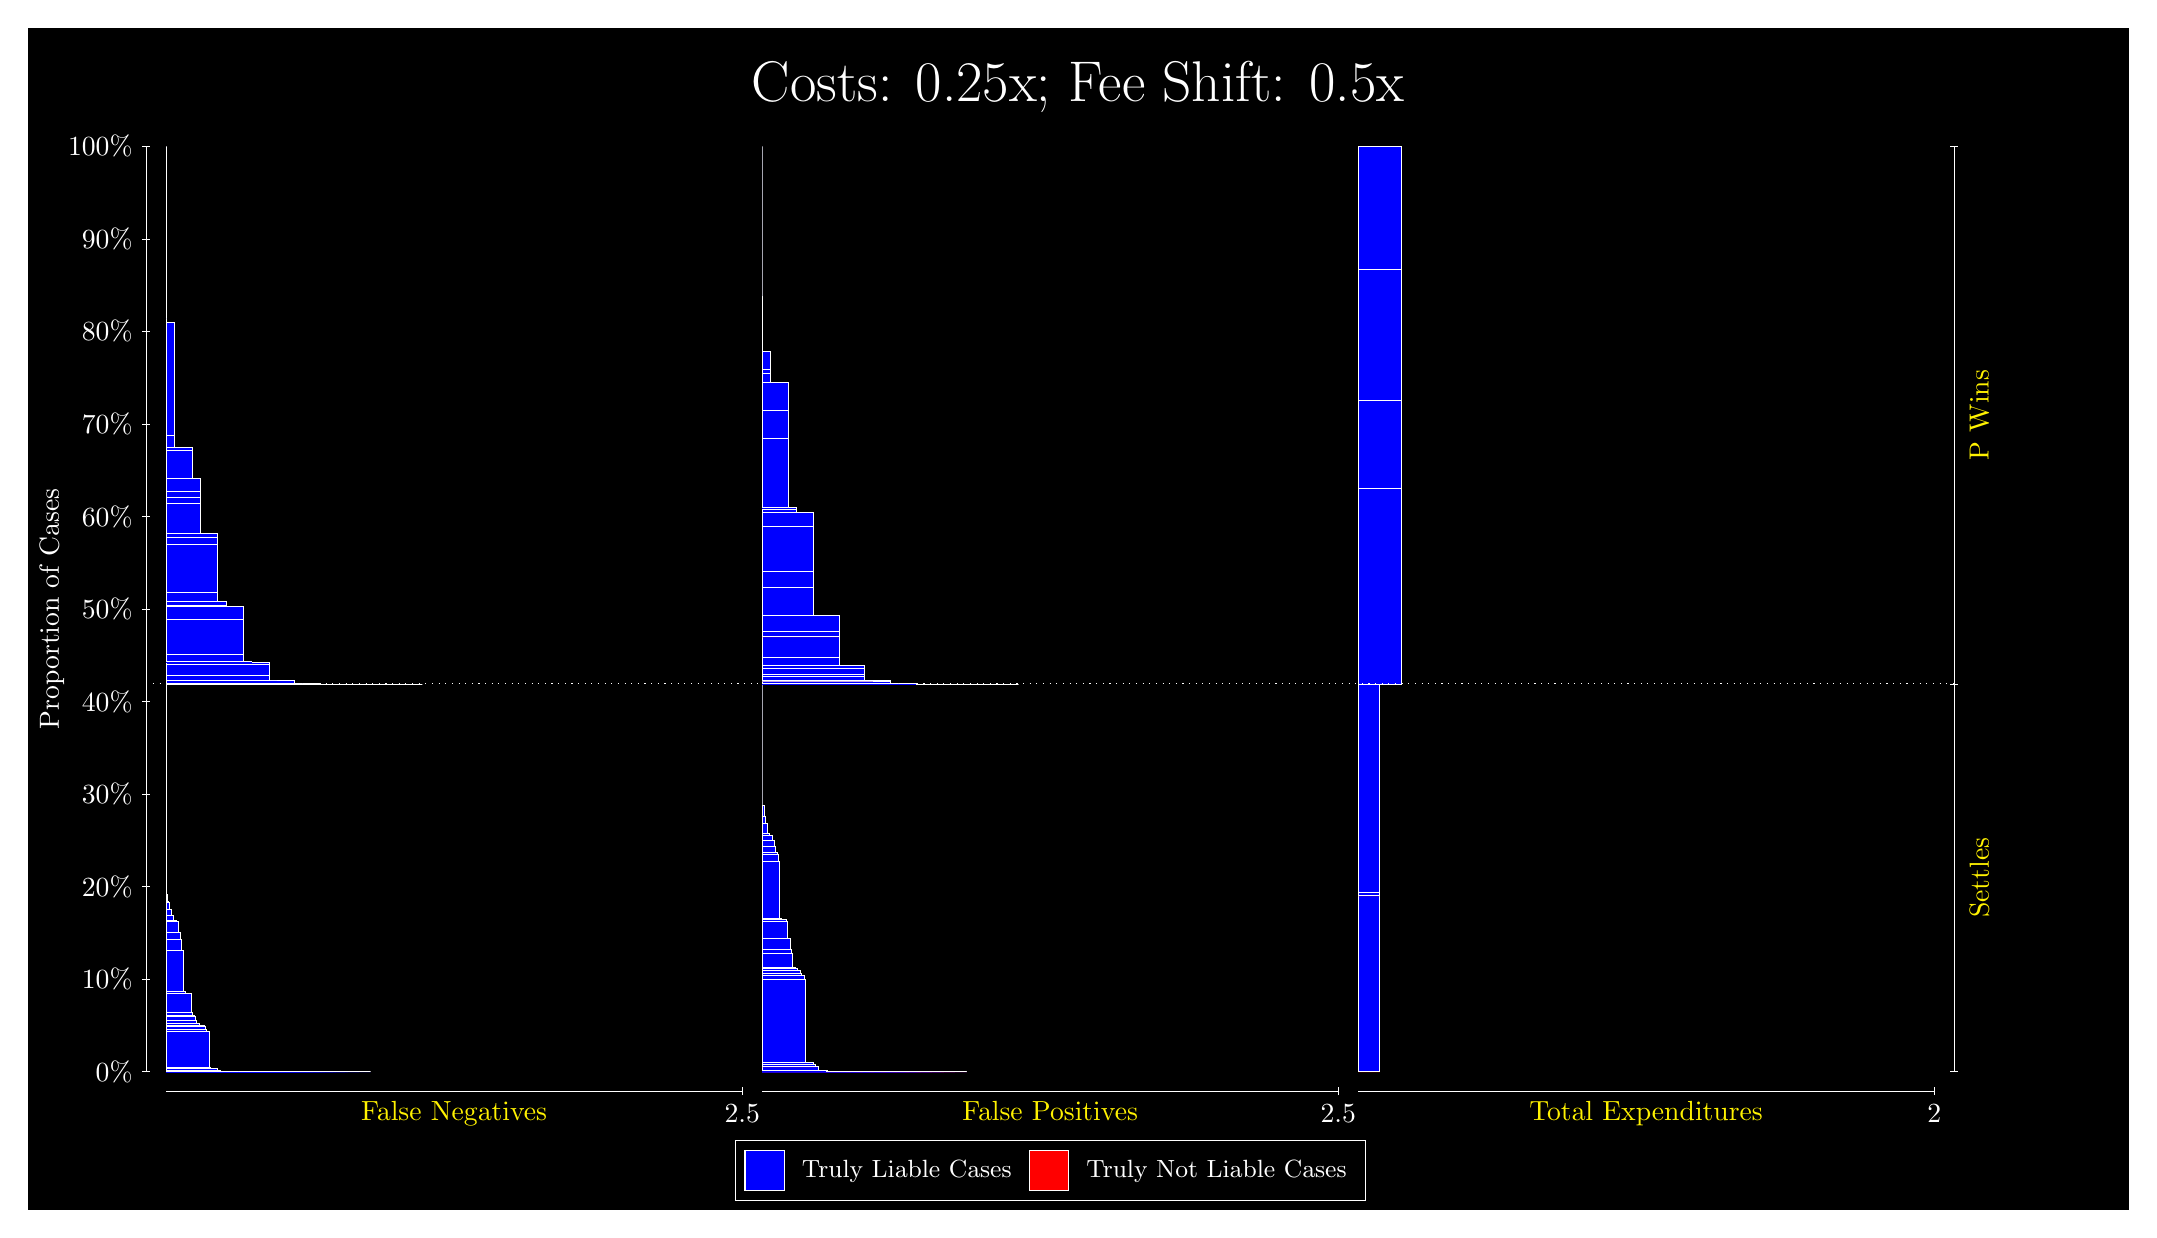
\begin{tikzpicture}
\draw[fill=black] (0,0) rectangle (26.667,15);
\draw[text=white] (0,13.5) rectangle (26.667,15) node[midway] {\huge Costs: 0.25x; Fee Shift: 0.5x};
\draw[white, very thin] (1.5,1.75) -- (1.5,13.5);
\node[rotate=90, text=white, anchor=center] at (0.3, 7.625) {Proportion of Cases};
\draw[white, very thin] (1.45,1.75) -- (1.55,1.75);
\node[text=white, anchor=east] at (1.45, 1.75) {0\%};
\draw[white, very thin] (1.45,2.925) -- (1.55,2.925);
\node[text=white, anchor=east] at (1.45, 2.925) {10\%};
\draw[white, very thin] (1.45,4.1) -- (1.55,4.1);
\node[text=white, anchor=east] at (1.45, 4.1) {20\%};
\draw[white, very thin] (1.45,5.275) -- (1.55,5.275);
\node[text=white, anchor=east] at (1.45, 5.275) {30\%};
\draw[white, very thin] (1.45,6.45) -- (1.55,6.45);
\node[text=white, anchor=east] at (1.45, 6.45) {40\%};
\draw[white, very thin] (1.45,7.625) -- (1.55,7.625);
\node[text=white, anchor=east] at (1.45, 7.625) {50\%};
\draw[white, very thin] (1.45,8.8) -- (1.55,8.8);
\node[text=white, anchor=east] at (1.45, 8.8) {60\%};
\draw[white, very thin] (1.45,9.975) -- (1.55,9.975);
\node[text=white, anchor=east] at (1.45, 9.975) {70\%};
\draw[white, very thin] (1.45,11.15) -- (1.55,11.15);
\node[text=white, anchor=east] at (1.45, 11.15) {80\%};
\draw[white, very thin] (1.45,12.325) -- (1.55,12.325);
\node[text=white, anchor=east] at (1.45, 12.325) {90\%};
\draw[white, very thin] (1.45,13.5) -- (1.55,13.5);
\node[text=white, anchor=east] at (1.45, 13.5) {100\%};

\draw[white, very thin] (24.457,1.75) -- (24.457,13.5);
\draw[white, very thin] (24.407,1.75) -- (24.507,1.75);
\node[anchor=west] at (24.407, 1.75) {};
\draw[white, very thin] (24.407,6.6736) -- (24.507,6.6736);
\node[anchor=west] at (24.407, 6.6736) {};
\draw[white, very thin] (24.407,13.5) -- (24.507,13.5);
\node[anchor=west] at (24.407, 13.5) {};

\draw[white, very thin, fill=blue] (1.75,1.75) rectangle (4.3482,1.75);
\draw[white, very thin, fill=blue] (1.75,1.75) rectangle (4.2018,1.75);
\draw[white, very thin, fill=blue] (1.75,1.75) rectangle (4.0554,1.75);
\draw[white, very thin, fill=blue] (1.75,1.75) rectangle (4.0229,1.75);
\draw[white, very thin, fill=blue] (1.75,1.75) rectangle (3.9091,1.75);
\draw[white, very thin, fill=blue] (1.75,1.75) rectangle (3.8765,1.75);
\draw[white, very thin, fill=blue] (1.75,1.75) rectangle (3.7627,1.75);
\draw[white, very thin, fill=blue] (1.75,1.75) rectangle (3.7302,1.75);
\draw[white, very thin, fill=blue] (1.75,1.75) rectangle (3.6976,1.75);
\draw[white, very thin, fill=blue] (1.75,1.75) rectangle (3.6163,1.75);
\draw[white, very thin, fill=blue] (1.75,1.75) rectangle (3.5838,1.75);
\draw[white, very thin, fill=blue] (1.75,1.75) rectangle (3.5513,1.75);
\draw[white, very thin, fill=blue] (1.75,1.75) rectangle (3.4699,1.75);
\draw[white, very thin, fill=blue] (1.75,1.75) rectangle (3.4374,1.75);
\draw[white, very thin, fill=blue] (1.75,1.75) rectangle (3.4049,1.75);
\draw[white, very thin, fill=blue] (1.75,1.75) rectangle (3.3723,1.75);
\draw[white, very thin, fill=blue] (1.75,1.75) rectangle (3.3236,1.75);
\draw[white, very thin, fill=blue] (1.75,1.75) rectangle (3.291,1.75);
\draw[white, very thin, fill=blue] (1.75,1.75) rectangle (3.2585,1.75);
\draw[white, very thin, fill=blue] (1.75,1.75) rectangle (3.226,1.75);
\draw[white, very thin, fill=blue] (1.75,1.75) rectangle (3.1772,1.75);
\draw[white, very thin, fill=blue] (1.75,1.75) rectangle (3.1447,1.75);
\draw[white, very thin, fill=blue] (1.75,1.75) rectangle (3.1121,1.75);
\draw[white, very thin, fill=blue] (1.75,1.75) rectangle (3.0796,1.75);
\draw[white, very thin, fill=blue] (1.75,1.75) rectangle (3.0471,1.75);
\draw[white, very thin, fill=blue] (1.75,1.75) rectangle (3.0308,1.75);
\draw[white, very thin, fill=blue] (1.75,1.75) rectangle (2.9983,1.75);
\draw[white, very thin, fill=blue] (1.75,1.75) rectangle (2.9657,1.75);
\draw[white, very thin, fill=blue] (1.75,1.75) rectangle (2.9332,1.75);
\draw[white, very thin, fill=blue] (1.75,1.75) rectangle (2.9007,1.75);
\draw[white, very thin, fill=blue] (1.75,1.75) rectangle (2.8844,1.75);
\draw[white, very thin, fill=blue] (1.75,1.75) rectangle (2.8519,1.75);
\draw[white, very thin, fill=blue] (1.75,1.75) rectangle (2.8194,1.75);
\draw[white, very thin, fill=blue] (1.75,1.75) rectangle (2.7868,1.7501);
\draw[white, very thin, fill=blue] (1.75,1.7501) rectangle (2.7543,1.7501);
\draw[white, very thin, fill=blue] (1.75,1.7501) rectangle (2.738,1.7502);
\draw[white, very thin, fill=blue] (1.75,1.7502) rectangle (2.7218,1.7506);
\draw[white, very thin, fill=blue] (1.75,1.7506) rectangle (2.7055,1.7506);
\draw[white, very thin, fill=blue] (1.75,1.7506) rectangle (2.673,1.7506);
\draw[white, very thin, fill=blue] (1.75,1.7506) rectangle (2.6405,1.7507);
\draw[white, very thin, fill=blue] (1.75,1.7507) rectangle (2.6079,1.7508);
\draw[white, very thin, fill=blue] (1.75,1.7508) rectangle (2.5917,1.7521);
\draw[white, very thin, fill=blue] (1.75,1.7521) rectangle (2.5754,1.7538);
\draw[white, very thin, fill=blue] (1.75,1.7538) rectangle (2.5591,1.7543);
\draw[white, very thin, fill=blue] (1.75,1.7543) rectangle (2.5266,1.7544);
\draw[white, very thin, fill=blue] (1.75,1.7544) rectangle (2.4941,1.7561);
\draw[white, very thin, fill=blue] (1.75,1.7561) rectangle (2.4616,1.7578);
\draw[white, very thin, fill=blue] (1.75,1.7578) rectangle (2.4453,1.767);
\draw[white, very thin, fill=blue] (1.75,1.767) rectangle (2.429,1.7698);
\draw[white, very thin, fill=blue] (1.75,1.7698) rectangle (2.4128,1.7718);
\draw[white, very thin, fill=blue] (1.75,1.7718) rectangle (2.3965,1.7959);
\draw[white, very thin, fill=blue] (1.75,1.7959) rectangle (2.3802,1.796);
\draw[white, very thin, fill=blue] (1.75,1.796) rectangle (2.3477,1.7961);
\draw[white, very thin, fill=blue] (1.75,1.7961) rectangle (2.3152,1.7989);
\draw[white, very thin, fill=blue] (1.75,1.7989) rectangle (2.2989,2.263);
\draw[white, very thin, fill=blue] (1.75,2.263) rectangle (2.2827,2.2648);
\draw[white, very thin, fill=blue] (1.75,2.2648) rectangle (2.2664,2.2898);
\draw[white, very thin, fill=blue] (1.75,2.2898) rectangle (2.2501,2.3197);
\draw[white, very thin, fill=blue] (1.75,2.3197) rectangle (2.2339,2.339);
\draw[white, very thin, fill=blue] (1.75,2.339) rectangle (2.2013,2.3417);
\draw[white, very thin, fill=blue] (1.75,2.3417) rectangle (2.1688,2.369);
\draw[white, very thin, fill=blue] (1.75,2.369) rectangle (2.1363,2.3963);
\draw[white, very thin, fill=blue] (1.75,2.3963) rectangle (2.12,2.4473);
\draw[white, very thin, fill=blue] (1.75,2.4473) rectangle (2.1037,2.4663);
\draw[white, very thin, fill=blue] (1.75,2.4663) rectangle (2.0875,2.4966);
\draw[white, very thin, fill=blue] (1.75,2.4966) rectangle (2.0712,2.7431);
\draw[white, very thin, fill=blue] (1.75,2.7431) rectangle (2.055,2.7448);
\draw[white, very thin, fill=blue] (1.75,2.7448) rectangle (2.0224,2.7465);
\draw[white, very thin, fill=blue] (1.75,2.7465) rectangle (1.9899,2.7642);
\draw[white, very thin, fill=blue] (1.75,2.7642) rectangle (1.9736,3.2906);
\draw[white, very thin, fill=blue] (1.75,3.2906) rectangle (1.9574,3.2954);
\draw[white, very thin, fill=blue] (1.75,3.2954) rectangle (1.9411,3.4294);
\draw[white, very thin, fill=blue] (1.75,3.4294) rectangle (1.9248,3.5164);
\draw[white, very thin, fill=blue] (1.75,3.5164) rectangle (1.9086,3.6529);
\draw[white, very thin, fill=blue] (1.75,3.6529) rectangle (1.876,3.6706);
\draw[white, very thin, fill=blue] (1.75,3.6706) rectangle (1.8435,3.7393);
\draw[white, very thin, fill=blue] (1.75,3.7393) rectangle (1.811,3.808);
\draw[white, very thin, fill=blue] (1.75,3.808) rectangle (1.7947,3.8949);
\draw[white, very thin, fill=blue] (1.75,3.8949) rectangle (1.7785,3.9167);
\draw[white, very thin, fill=blue] (1.75,3.9167) rectangle (1.7622,4.0026);
\draw[white, very thin, fill=red] (1.75,4.0026) rectangle (1.75,4.0026);
\draw[white, very thin, fill=blue] (1.75,4.0026) rectangle (1.75,6.6736);
\draw[white, very thin, fill=blue] (1.75,6.6736) rectangle (5.0069,6.6736);
\draw[white, very thin, fill=blue] (1.75,6.6736) rectangle (4.6816,6.6736);
\draw[white, very thin, fill=blue] (1.75,6.6736) rectangle (4.3563,6.6736);
\draw[white, very thin, fill=blue] (1.75,6.6736) rectangle (4.1368,6.6736);
\draw[white, very thin, fill=blue] (1.75,6.6736) rectangle (4.031,6.6739);
\draw[white, very thin, fill=blue] (1.75,6.6739) rectangle (4.031,6.674);
\draw[white, very thin, fill=blue] (1.75,6.674) rectangle (3.8115,6.674);
\draw[white, very thin, fill=blue] (1.75,6.674) rectangle (3.7058,6.6773);
\draw[white, very thin, fill=blue] (1.75,6.6773) rectangle (3.7058,6.6791);
\draw[white, very thin, fill=blue] (1.75,6.6791) rectangle (3.4862,6.6791);
\draw[white, very thin, fill=blue] (1.75,6.6791) rectangle (3.4862,6.6791);
\draw[white, very thin, fill=blue] (1.75,6.6791) rectangle (3.3805,6.7225);
\draw[white, very thin, fill=blue] (1.75,6.7225) rectangle (3.1609,6.7225);
\draw[white, very thin, fill=blue] (1.75,6.7225) rectangle (3.1609,6.7225);
\draw[white, very thin, fill=blue] (1.75,6.7225) rectangle (3.0552,6.7822);
\draw[white, very thin, fill=blue] (1.75,6.7822) rectangle (3.0552,6.9274);
\draw[white, very thin, fill=blue] (1.75,6.9274) rectangle (3.0552,6.9528);
\draw[white, very thin, fill=blue] (1.75,6.9528) rectangle (2.8356,6.954);
\draw[white, very thin, fill=blue] (1.75,6.954) rectangle (2.8356,6.9543);
\draw[white, very thin, fill=blue] (1.75,6.9543) rectangle (2.8356,6.9547);
\draw[white, very thin, fill=blue] (1.75,6.9547) rectangle (2.7299,7.0429);
\draw[white, very thin, fill=blue] (1.75,7.0429) rectangle (2.7299,7.4902);
\draw[white, very thin, fill=blue] (1.75,7.4902) rectangle (2.7299,7.6576);
\draw[white, very thin, fill=blue] (1.75,7.6576) rectangle (2.5103,7.6664);
\draw[white, very thin, fill=blue] (1.75,7.6664) rectangle (2.5103,7.7238);
\draw[white, very thin, fill=blue] (1.75,7.7238) rectangle (2.4046,7.8319);
\draw[white, very thin, fill=blue] (1.75,7.8319) rectangle (2.4046,8.4436);
\draw[white, very thin, fill=blue] (1.75,8.4436) rectangle (2.4046,8.5286);
\draw[white, very thin, fill=blue] (1.75,8.5286) rectangle (2.4046,8.5796);
\draw[white, very thin, fill=blue] (1.75,8.5796) rectangle (2.1851,8.9664);
\draw[white, very thin, fill=blue] (1.75,8.9664) rectangle (2.1851,9.0384);
\draw[white, very thin, fill=blue] (1.75,9.0384) rectangle (2.1851,9.1145);
\draw[white, very thin, fill=blue] (1.75,9.1145) rectangle (2.1851,9.283);
\draw[white, very thin, fill=blue] (1.75,9.283) rectangle (2.0793,9.6451);
\draw[white, very thin, fill=blue] (1.75,9.6451) rectangle (2.0793,9.6743);
\draw[white, very thin, fill=blue] (1.75,9.6743) rectangle (1.8598,9.8289);
\draw[white, very thin, fill=blue] (1.75,9.8289) rectangle (1.8598,11.262);
\draw[white, very thin, fill=blue] (1.75,11.262) rectangle (1.7541,11.317);
\draw[white, very thin, fill=blue] (1.75,11.317) rectangle (1.7541,11.318);
\draw[white, very thin, fill=blue] (1.75,11.318) rectangle (1.7541,11.318);
\draw[white, very thin, fill=red] (1.75,11.318) rectangle (1.75,11.318);
\draw[white, very thin, fill=blue] (1.75,11.318) rectangle (1.75,13.5);
\draw[white, very thin, fill=red] (9.3189,1.75) rectangle (11.917,1.75);
\draw[white, very thin, fill=blue] (9.3189,1.75) rectangle (11.917,1.75);
\draw[white, very thin, fill=red] (9.3189,1.75) rectangle (11.771,1.75);
\draw[white, very thin, fill=blue] (9.3189,1.75) rectangle (11.771,1.75);
\draw[white, very thin, fill=red] (9.3189,1.75) rectangle (11.624,1.75);
\draw[white, very thin, fill=blue] (9.3189,1.75) rectangle (11.624,1.75);
\draw[white, very thin, fill=blue] (9.3189,1.75) rectangle (11.592,1.75);
\draw[white, very thin, fill=red] (9.3189,1.75) rectangle (11.478,1.75);
\draw[white, very thin, fill=blue] (9.3189,1.75) rectangle (11.478,1.75);
\draw[white, very thin, fill=blue] (9.3189,1.75) rectangle (11.445,1.75);
\draw[white, very thin, fill=red] (9.3189,1.75) rectangle (11.332,1.75);
\draw[white, very thin, fill=blue] (9.3189,1.75) rectangle (11.332,1.75);
\draw[white, very thin, fill=blue] (9.3189,1.75) rectangle (11.299,1.75);
\draw[white, very thin, fill=blue] (9.3189,1.75) rectangle (11.266,1.75);
\draw[white, very thin, fill=red] (9.3189,1.75) rectangle (11.185,1.75);
\draw[white, very thin, fill=blue] (9.3189,1.75) rectangle (11.185,1.75);
\draw[white, very thin, fill=blue] (9.3189,1.75) rectangle (11.153,1.75);
\draw[white, very thin, fill=blue] (9.3189,1.75) rectangle (11.12,1.75);
\draw[white, very thin, fill=red] (9.3189,1.75) rectangle (11.039,1.75);
\draw[white, very thin, fill=blue] (9.3189,1.75) rectangle (11.039,1.75);
\draw[white, very thin, fill=blue] (9.3189,1.75) rectangle (11.006,1.75);
\draw[white, very thin, fill=blue] (9.3189,1.75) rectangle (10.974,1.75);
\draw[white, very thin, fill=blue] (9.3189,1.75) rectangle (10.941,1.75);
\draw[white, very thin, fill=red] (9.3189,1.75) rectangle (10.892,1.75);
\draw[white, very thin, fill=blue] (9.3189,1.75) rectangle (10.892,1.75);
\draw[white, very thin, fill=blue] (9.3189,1.75) rectangle (10.86,1.75);
\draw[white, very thin, fill=blue] (9.3189,1.75) rectangle (10.827,1.75);
\draw[white, very thin, fill=blue] (9.3189,1.75) rectangle (10.795,1.75);
\draw[white, very thin, fill=red] (9.3189,1.75) rectangle (10.746,1.75);
\draw[white, very thin, fill=blue] (9.3189,1.75) rectangle (10.746,1.75);
\draw[white, very thin, fill=blue] (9.3189,1.75) rectangle (10.714,1.75);
\draw[white, very thin, fill=blue] (9.3189,1.75) rectangle (10.681,1.75);
\draw[white, very thin, fill=blue] (9.3189,1.75) rectangle (10.648,1.75);
\draw[white, very thin, fill=blue] (9.3189,1.75) rectangle (10.616,1.75);
\draw[white, very thin, fill=red] (9.3189,1.75) rectangle (10.6,1.75);
\draw[white, very thin, fill=blue] (9.3189,1.75) rectangle (10.6,1.75);
\draw[white, very thin, fill=blue] (9.3189,1.75) rectangle (10.567,1.75);
\draw[white, very thin, fill=blue] (9.3189,1.75) rectangle (10.535,1.75);
\draw[white, very thin, fill=blue] (9.3189,1.75) rectangle (10.502,1.7501);
\draw[white, very thin, fill=blue] (9.3189,1.7501) rectangle (10.47,1.7501);
\draw[white, very thin, fill=red] (9.3189,1.7501) rectangle (10.453,1.7501);
\draw[white, very thin, fill=blue] (9.3189,1.7501) rectangle (10.453,1.7502);
\draw[white, very thin, fill=blue] (9.3189,1.7502) rectangle (10.421,1.7502);
\draw[white, very thin, fill=blue] (9.3189,1.7502) rectangle (10.388,1.7502);
\draw[white, very thin, fill=blue] (9.3189,1.7502) rectangle (10.356,1.7524);
\draw[white, very thin, fill=blue] (9.3189,1.7524) rectangle (10.323,1.753);
\draw[white, very thin, fill=red] (9.3189,1.753) rectangle (10.307,1.753);
\draw[white, very thin, fill=blue] (9.3189,1.753) rectangle (10.307,1.753);
\draw[white, very thin, fill=blue] (9.3189,1.753) rectangle (10.291,1.7535);
\draw[white, very thin, fill=blue] (9.3189,1.7535) rectangle (10.274,1.7535);
\draw[white, very thin, fill=blue] (9.3189,1.7535) rectangle (10.242,1.7536);
\draw[white, very thin, fill=blue] (9.3189,1.7536) rectangle (10.209,1.7537);
\draw[white, very thin, fill=blue] (9.3189,1.7537) rectangle (10.177,1.7581);
\draw[white, very thin, fill=red] (9.3189,1.7581) rectangle (10.161,1.7581);
\draw[white, very thin, fill=blue] (9.3189,1.7581) rectangle (10.161,1.7585);
\draw[white, very thin, fill=blue] (9.3189,1.7585) rectangle (10.144,1.7602);
\draw[white, very thin, fill=blue] (9.3189,1.7602) rectangle (10.128,1.7622);
\draw[white, very thin, fill=blue] (9.3189,1.7622) rectangle (10.095,1.7639);
\draw[white, very thin, fill=blue] (9.3189,1.7639) rectangle (10.063,1.7667);
\draw[white, very thin, fill=blue] (9.3189,1.7667) rectangle (10.03,1.8112);
\draw[white, very thin, fill=red] (9.3189,1.8112) rectangle (10.014,1.8112);
\draw[white, very thin, fill=blue] (9.3189,1.8112) rectangle (10.014,1.8204);
\draw[white, very thin, fill=blue] (9.3189,1.8204) rectangle (9.9979,1.8422);
\draw[white, very thin, fill=blue] (9.3189,1.8422) rectangle (9.9816,1.8423);
\draw[white, very thin, fill=blue] (9.3189,1.8423) rectangle (9.9654,1.866);
\draw[white, very thin, fill=blue] (9.3189,1.866) rectangle (9.9491,1.8688);
\draw[white, very thin, fill=blue] (9.3189,1.8688) rectangle (9.9166,1.8705);
\draw[white, very thin, fill=blue] (9.3189,1.8705) rectangle (9.884,1.8722);
\draw[white, very thin, fill=red] (9.3189,1.8722) rectangle (9.8678,1.8722);
\draw[white, very thin, fill=blue] (9.3189,1.8722) rectangle (9.8678,2.9242);
\draw[white, very thin, fill=blue] (9.3189,2.9242) rectangle (9.8515,2.9686);
\draw[white, very thin, fill=blue] (9.3189,2.9686) rectangle (9.8353,2.9737);
\draw[white, very thin, fill=blue] (9.3189,2.9737) rectangle (9.819,3.0036);
\draw[white, very thin, fill=blue] (9.3189,3.0036) rectangle (9.8027,3.0312);
\draw[white, very thin, fill=blue] (9.3189,3.0312) rectangle (9.7702,3.0585);
\draw[white, very thin, fill=blue] (9.3189,3.0585) rectangle (9.7377,3.0762);
\draw[white, very thin, fill=blue] (9.3189,3.0762) rectangle (9.7051,3.254);
\draw[white, very thin, fill=blue] (9.3189,3.254) rectangle (9.6889,3.3051);
\draw[white, very thin, fill=blue] (9.3189,3.3051) rectangle (9.6726,3.4376);
\draw[white, very thin, fill=blue] (9.3189,3.4376) rectangle (9.6563,3.4397);
\draw[white, very thin, fill=blue] (9.3189,3.4397) rectangle (9.6401,3.6644);
\draw[white, very thin, fill=blue] (9.3189,3.6644) rectangle (9.6238,3.6821);
\draw[white, very thin, fill=blue] (9.3189,3.6821) rectangle (9.5913,3.6864);
\draw[white, very thin, fill=blue] (9.3189,3.6864) rectangle (9.5588,3.6908);
\draw[white, very thin, fill=blue] (9.3189,3.6908) rectangle (9.5425,4.421);
\draw[white, very thin, fill=blue] (9.3189,4.421) rectangle (9.5262,4.5069);
\draw[white, very thin, fill=blue] (9.3189,4.5069) rectangle (9.51,4.5287);
\draw[white, very thin, fill=blue] (9.3189,4.5287) rectangle (9.4937,4.6156);
\draw[white, very thin, fill=blue] (9.3189,4.6156) rectangle (9.4774,4.6843);
\draw[white, very thin, fill=blue] (9.3189,4.6843) rectangle (9.4449,4.753);
\draw[white, very thin, fill=blue] (9.3189,4.753) rectangle (9.4124,4.7707);
\draw[white, very thin, fill=blue] (9.3189,4.7707) rectangle (9.3799,4.9072);
\draw[white, very thin, fill=blue] (9.3189,4.9072) rectangle (9.3636,4.9942);
\draw[white, very thin, fill=blue] (9.3189,4.9942) rectangle (9.3473,5.1282);
\draw[white, very thin, fill=blue] (9.3189,5.1282) rectangle (9.3311,5.133);
\draw[white, very thin, fill=blue] (9.3189,5.133) rectangle (9.3189,6.6736);
\draw[white, very thin, fill=red] (9.3189,6.6736) rectangle (12.576,6.6736);
\draw[white, very thin, fill=blue] (9.3189,6.6736) rectangle (12.576,6.6736);
\draw[white, very thin, fill=red] (9.3189,6.6736) rectangle (12.25,6.6736);
\draw[white, very thin, fill=blue] (9.3189,6.6736) rectangle (12.25,6.6736);
\draw[white, very thin, fill=blue] (9.3189,6.6736) rectangle (11.925,6.6736);
\draw[white, very thin, fill=red] (9.3189,6.6736) rectangle (11.925,6.6736);
\draw[white, very thin, fill=blue] (9.3189,6.6736) rectangle (11.925,6.6736);
\draw[white, very thin, fill=red] (9.3189,6.6736) rectangle (11.706,6.6736);
\draw[white, very thin, fill=blue] (9.3189,6.6736) rectangle (11.706,6.6736);
\draw[white, very thin, fill=blue] (9.3189,6.6736) rectangle (11.6,6.6738);
\draw[white, very thin, fill=blue] (9.3189,6.6738) rectangle (11.6,6.6738);
\draw[white, very thin, fill=red] (9.3189,6.6738) rectangle (11.6,6.6738);
\draw[white, very thin, fill=blue] (9.3189,6.6738) rectangle (11.6,6.6739);
\draw[white, very thin, fill=red] (9.3189,6.6739) rectangle (11.38,6.6739);
\draw[white, very thin, fill=blue] (9.3189,6.6739) rectangle (11.38,6.6739);
\draw[white, very thin, fill=red] (9.3189,6.6739) rectangle (11.275,6.6739);
\draw[white, very thin, fill=blue] (9.3189,6.6739) rectangle (11.275,6.6766);
\draw[white, very thin, fill=blue] (9.3189,6.6766) rectangle (11.275,6.6776);
\draw[white, very thin, fill=blue] (9.3189,6.6776) rectangle (11.275,6.6781);
\draw[white, very thin, fill=red] (9.3189,6.6781) rectangle (11.055,6.6781);
\draw[white, very thin, fill=blue] (9.3189,6.6781) rectangle (11.055,6.6781);
\draw[white, very thin, fill=blue] (9.3189,6.6781) rectangle (11.055,6.6781);
\draw[white, very thin, fill=red] (9.3189,6.6781) rectangle (10.949,6.6781);
\draw[white, very thin, fill=blue] (9.3189,6.6781) rectangle (10.949,6.7076);
\draw[white, very thin, fill=blue] (9.3189,6.7076) rectangle (10.949,6.7146);
\draw[white, very thin, fill=blue] (9.3189,6.7146) rectangle (10.73,6.7146);
\draw[white, very thin, fill=red] (9.3189,6.7146) rectangle (10.73,6.7146);
\draw[white, very thin, fill=blue] (9.3189,6.7146) rectangle (10.73,6.7146);
\draw[white, very thin, fill=blue] (9.3189,6.7146) rectangle (10.624,6.7751);
\draw[white, very thin, fill=blue] (9.3189,6.7751) rectangle (10.624,6.7925);
\draw[white, very thin, fill=red] (9.3189,6.7925) rectangle (10.624,6.7925);
\draw[white, very thin, fill=blue] (9.3189,6.7925) rectangle (10.624,6.8699);
\draw[white, very thin, fill=blue] (9.3189,6.8699) rectangle (10.624,6.9073);
\draw[white, very thin, fill=blue] (9.3189,6.9073) rectangle (10.404,6.9073);
\draw[white, very thin, fill=red] (9.3189,6.9073) rectangle (10.404,6.9073);
\draw[white, very thin, fill=blue] (9.3189,6.9073) rectangle (10.404,6.9073);
\draw[white, very thin, fill=blue] (9.3189,6.9073) rectangle (10.299,7.0167);
\draw[white, very thin, fill=blue] (9.3189,7.0167) rectangle (10.299,7.2723);
\draw[white, very thin, fill=red] (9.3189,7.2723) rectangle (10.299,7.2723);
\draw[white, very thin, fill=blue] (9.3189,7.2723) rectangle (10.299,7.3429);
\draw[white, very thin, fill=blue] (9.3189,7.3429) rectangle (10.299,7.5488);
\draw[white, very thin, fill=blue] (9.3189,7.5488) rectangle (10.079,7.5488);
\draw[white, very thin, fill=red] (9.3189,7.5488) rectangle (10.079,7.5488);
\draw[white, very thin, fill=blue] (9.3189,7.5488) rectangle (10.079,7.5491);
\draw[white, very thin, fill=blue] (9.3189,7.5491) rectangle (9.9735,7.898);
\draw[white, very thin, fill=blue] (9.3189,7.898) rectangle (9.9735,8.1013);
\draw[white, very thin, fill=blue] (9.3189,8.1013) rectangle (9.9735,8.6726);
\draw[white, very thin, fill=blue] (9.3189,8.6726) rectangle (9.9735,8.8559);
\draw[white, very thin, fill=blue] (9.3189,8.8559) rectangle (9.7539,8.857);
\draw[white, very thin, fill=red] (9.3189,8.857) rectangle (9.7539,8.857);
\draw[white, very thin, fill=blue] (9.3189,8.857) rectangle (9.7539,8.8949);
\draw[white, very thin, fill=blue] (9.3189,8.8949) rectangle (9.7539,8.9111);
\draw[white, very thin, fill=blue] (9.3189,8.9111) rectangle (9.7539,8.9121);
\draw[white, very thin, fill=blue] (9.3189,8.9121) rectangle (9.6482,9.7872);
\draw[white, very thin, fill=blue] (9.3189,9.7872) rectangle (9.6482,10.142);
\draw[white, very thin, fill=blue] (9.3189,10.142) rectangle (9.6482,10.499);
\draw[white, very thin, fill=blue] (9.3189,10.499) rectangle (9.4287,10.619);
\draw[white, very thin, fill=red] (9.3189,10.619) rectangle (9.4287,10.619);
\draw[white, very thin, fill=blue] (9.3189,10.619) rectangle (9.4287,10.666);
\draw[white, very thin, fill=blue] (9.3189,10.666) rectangle (9.4287,10.891);
\draw[white, very thin, fill=blue] (9.3189,10.891) rectangle (9.3229,10.967);
\draw[white, very thin, fill=blue] (9.3189,10.967) rectangle (9.3229,11.518);
\draw[white, very thin, fill=blue] (9.3189,11.518) rectangle (9.3229,11.594);
\draw[white, very thin, fill=blue] (9.3189,11.594) rectangle (9.3189,13.5);
\draw[white, very thin, fill=red] (16.888,1.75) rectangle (17.162,1.75);
\draw[white, very thin, fill=blue] (16.888,1.75) rectangle (17.162,3.9822);
\draw[white, very thin, fill=red] (16.888,3.9822) rectangle (17.162,3.9822);
\draw[white, very thin, fill=blue] (16.888,3.9822) rectangle (17.162,4.0311);
\draw[white, very thin, fill=red] (16.888,4.0311) rectangle (17.162,4.0311);
\draw[white, very thin, fill=blue] (16.888,4.0311) rectangle (17.162,6.6736);
\draw[white, very thin, fill=red] (16.888,6.6736) rectangle (17.437,6.6736);
\draw[white, very thin, fill=blue] (16.888,6.6736) rectangle (17.437,9.1571);
\draw[white, very thin, fill=red] (16.888,9.1571) rectangle (17.437,9.1571);
\draw[white, very thin, fill=blue] (16.888,9.1571) rectangle (17.437,10.272);
\draw[white, very thin, fill=red] (16.888,10.272) rectangle (17.437,10.272);
\draw[white, very thin, fill=blue] (16.888,10.272) rectangle (17.437,11.936);
\draw[white, very thin, fill=red] (16.888,11.936) rectangle (17.437,11.936);
\draw[white, very thin, fill=blue] (16.888,11.936) rectangle (17.437,13.5);
\draw[white, dotted] (1.5,6.6736) -- (24.457,6.6736);
\draw[white, very thin] (1.75,1.5) -- (9.0689,1.5);
\node[text=yellow, anchor=north] at (5.4094, 1.5) {False Negatives};
\draw[white, very thin] (9.0689,1.45) -- (9.0689,1.55);
\node[text=white, anchor=north] at (9.0689, 1.45) {2.5};

\draw[white, very thin] (9.3189,1.5) -- (16.638,1.5);
\node[text=yellow, anchor=north] at (12.978, 1.5) {False Positives};
\draw[white, very thin] (16.638,1.45) -- (16.638,1.55);
\node[text=white, anchor=north] at (16.638, 1.45) {2.5};

\draw[white, very thin] (16.888,1.5) -- (24.207,1.5);
\node[text=yellow, anchor=north] at (20.547, 1.5) {Total Expenditures};
\draw[white, very thin] (24.207,1.45) -- (24.207,1.55);
\node[text=white, anchor=north] at (24.207, 1.45) {2};

\node[text=yellow, centered, rotate=90] at (24.777, 4.2118) {Settles};
\node[text=yellow, centered, rotate=90] at (24.777, 10.087) {P Wins};

\draw (12.978300999999998,1.5) node[draw=none] (baseCoordinate) {};
\begin{scope}[align=center]
        \matrix[scale=0.5, draw=white, below=0.5cm of baseCoordinate, nodes={draw}, column sep=0.1cm]{
            \node[rectangle, draw, minimum width=0.5cm, minimum height=0.5cm, fill=blue] {}; &
            \node[draw=none, font=\small, text=white] (B) {Truly Liable Cases}; &
            \node[rectangle, draw, minimum width=0.5cm, minimum height=0.5cm, fill=red] {}; &
            \node[draw=none, font=\small, text=white] (B) {Truly Not Liable Cases}; \\
            };
\end{scope}

\end{tikzpicture}
\end{document}